\chapter{Planning d'Urgence Commando : J-4 jusqu'au 27 Septembre}

Avec quatre jours avant les épreuves écrites du \textbf{dimanche 27 septembre 2026} (présence à \textbf{7h30} à la \textbf{FSJES de Salé}, route Outa Hssain, Salé El Jadida, avec la CIN), la stratégie est celle du \textbf{haut rendement ciblé}. Le barème impose les priorités : l'épreuve de \textbf{spécialité informatique et réseaux (3 h, coefficient 4)} pèse deux fois plus que la \textbf{rédaction sur les attributions du ministère (2 h, coefficient 2)}. Il faut donc consacrer environ 60 \% du temps à la spécialité (réseaux et télécommunications en priorité, développement ensuite) et 40 \% à la matière diplomatique, tout en capitalisant sur la méthode acquise pour le MEF (plan binaire, introduction en 5 étapes).

\begin{tcolorbox}[colback=blue!5!white,colframe=blue!75!black,title=\textbf{Ce qui est déjà acquis (ne pas y repasser du temps)}]
La méthodologie de la dissertation (à recaler sur 2 heures), la structure en deux parties, le socle informatique général (algorithmique, SQL, POO, cybersécurité, data) et la culture économique générale (PIB, déficit, dette, inflation). Une relecture rapide suffit ; l'effort nouveau porte sur les réseaux et télécommunications, qui n'étaient qu'un bloc parmi d'autres au MEF et deviennent ici la spécialité la plus dotée (10 postes sur 16).
\end{tcolorbox}

\section{Le Programme Heure par Heure (Sprint Final)}

\begin{table}[H]
\centering
\small
\begin{tabular}{|p{3cm}|p{3.5cm}|p{8.5cm}|}
\hline
\rowcolor{gray!20} \textbf{Jour / Date} & \textbf{Créneau Horaire} & \textbf{Objectif Haute Rentabilité} \\ \hline
\multirow{2}{*}{\textbf{J-4 : 23 Sept.}} & 15h00 - 19h00 & \textbf{Bloc 1 : Cadrage du concours et fondamentaux de la diplomatie marocaine} \newline Lire l'introduction et le chapitre 1 (les trois épreuves, barème, attentes du jury). Mémoriser la Fiche 1 (organisation du MAECAME) et la Fiche 2 (constantes de la politique étrangère). \\ \cline{2-3}
& 20h00 - 23h00 & \textbf{Bloc 2 : Spécialité --- Réseaux et télécommunications (1)} \newline Modèle OSI/TCP-IP, adressage et sous-réseaux (exercices de calcul), routage, VLAN, VPN, Wi-Fi, sécurité périmétrique. Traiter les exercices rédigés du chapitre 3 (architecture réseau d'une ambassade). \\ \hline

\multirow{3}{*}{\textbf{J-3 : 24 Sept.}} & 08h30 - 12h30 & \textbf{Bloc 3 : Spécialité --- Développement et bases de données} \newline POO, architecture web et API, SQL et Merise (exercice de conception d'un système de rendez-vous consulaire), génie logiciel, sécurité applicative (OWASP). \\ \cline{2-3}
& 14h00 - 18h00 & \textbf{Bloc 4 : Sahara, Afrique et Marocains du monde} \newline Fiches 3, 4 et 5 : chronologie du Sahara et résolution 2797, retour à l'UA, Initiative Atlantique, gazoduc, chiffres MRE et réforme de 2024. Lire les Sujets 1 à 3 du chapitre 2. \\ \cline{2-3}
& 19h00 - 22h30 & \textbf{Bloc 5 : Simulation de la rédaction en 2 h chrono} \newline Rédiger un sujet du chapitre 2 \textbf{sans regarder la copie modèle}, puis se corriger avec la grille. Ensuite, lire les Sujets 4 à 6 (diplomatie économique, numérique consulaire, multilatéralisme). \\ \hline

\multirow{3}{*}{\textbf{J-2 : 25 Sept.}} & 09h00 - 12h30 & \textbf{Bloc 6 : Spécialité --- Réseaux et télécommunications (2)} \newline Télécoms (fibre, 4G/5G, VoIP, liaisons satellitaires pour les postes isolés), supervision, haute disponibilité, PRA/PCA, cybersécurité (loi 05-20, DNSSI, ISO 27001). Refaire les calculs de sous-réseaux. \\ \cline{2-3}
& 14h30 - 17h30 & \textbf{Bloc 7 : Banque de questions ministère et diplomatie} \newline Parcourir toutes les questions 🔴 et 🟠 du chapitre 3 en cachant les réponses ; relire les Fiches 6 et 7. \\ \cline{2-3}
& 18h30 - 21h00 & \textbf{Bloc 8 : Examen blanc complet (chapitre 6)} \newline Épreuve de spécialité (3 h) puis, après une pause, la rédaction (2 h) ; autocorrection avec les grilles. \\ \hline

\multirow{2}{*}{\textbf{J-1 : 26 Sept.}} & 09h00 - 12h00 & \textbf{Bloc 9 : Fiches chiffres clés et phrases d'accroche} \newline Mémoriser la Fiche 8 (dates et chiffres), les pièges du chapitre 3 et préparer 5 accroches réutilisables (discours royaux, résolution 2797, Constitution). \\ \cline{2-3}
& 14h00 - 17h00 & \textbf{Bloc 10 : Préparation matérielle et sérénité} \newline CIN obligatoire (l'annonce officielle tient lieu de convocation), numéro de salle et de siège notés, stylos, montre analogique, calculatrice simple si autorisée, trajet vers la FSJES de Salé repéré. \textbf{Arrêt complet des révisions à 18h00.} \\ \hline

\textbf{Jour J : 27 Sept.} & 07h30 & \textbf{Épreuves écrites à la FSJES de Salé} \newline Arrivée à 7h00. Spécialité (3 h) : lire tout le sujet, traiter d'abord les questions sûres, garder 15 minutes de relecture. Rédaction (2 h) : timing 10m / 20m / 10m / 70m / 10m. \\ \hline
\end{tabular}
\caption{Planning intensif d'urgence J-4}
\end{table}

\IfFileExists{images/img_012_planning_commando_j4_matrice.png}{%
\begin{figure}[H]
    \centering
    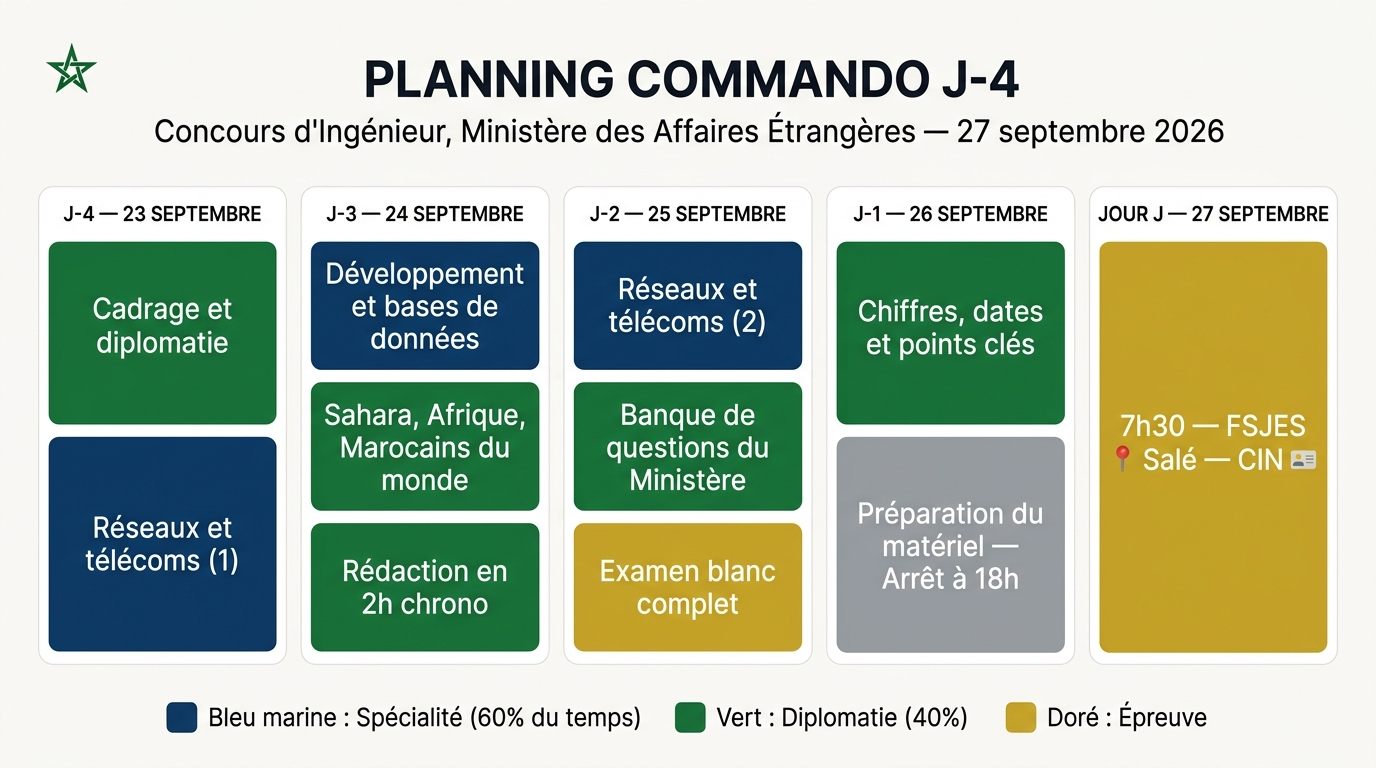
\includegraphics[width=\textwidth]{images/img_012_planning_commando_j4_matrice.png}
    \caption{Matrice d'urgence des 4 jours avant l'épreuve du 27 septembre}
\end{figure}}{}

\section{Checklist Finale pour le Jour J}
\begin{enumerate}
    \item \textbf{Vocabulaire valorisé :} \textit{intégrité territoriale, plan d'autonomie, diplomatie économique, coopération Sud-Sud, partenariat gagnant-gagnant, co-développement, voisinage, multilatéralisme, diplomatie de proximité au service des Marocains du monde, souveraineté numérique, protection des données.}
    \item \textbf{Références à mobiliser :} discours royaux (Marche Verte, Trône, Révolution du Roi et du Peuple), Constitution de 2011 (préambule sur l'appartenance africaine et arabo-islamique, articles 16 à 18 sur les MRE), résolutions du Conseil de sécurité, Acte constitutif de l'Union Africaine.
    \item \textbf{Posture d'ingénieur d'État :} montrer que la technologie sert la diplomatie : services consulaires numériques, sécurité des systèmes d'information, données des Marocains du monde, communication et image du Royaume.
    \item \textbf{Neutralité et rigueur :} ton institutionnel, pas de polémique, pas de chiffre inventé ; en cas de doute, formuler avec prudence (« selon les données officielles récentes »).
\end{enumerate}
